%% AZIENDA OSPITANTE
\chapter{Azienda ospitante}\label{chap:company}

\section{Profilo dell'azienda}
L'attività di stage descritta in questo elaborato è stata svolta presso l'azienda Zextras s.r.l. con sede a  \unsure{Vicenza}. Essa è nata nel 2011 con l'obbiettivo di espandere le possibilità del software Zimbra.
\mmh{...}{scrivere altro}

\subsection{Zimbra}
\postit{Questa parte in cui parli dei software dell'azienda potrebbe essere spostata nella sezione delle tecnologie}
Zimbra è una suite di software collaborativi open source che consente di condividere documenti e attività.  \mmh{...}{scrivere altro}\\
Essa offre:
\begin{itemize}
	\item[•] configurazione personalizzata
	\item[•] gestione della posta elettronica
	\item[•] rubriche, calendari e condivisione di file
	\item[•] chat e chiamate vocali
	\item[•] integrazione con i canali web
	\item[•] privacy e alti livelli di sicurezza
	\item[•] disponibilità per i dispositivi mobili: oltre che mediante client Zimbra Web e attraverso i client di posta elettronica tradizionale, è possibile accedere alle e-mail, ai calendari e alle altre offerte da dispositivi mobile. 
\end{itemize}
Zimbra è disponibile in due versioni: Zimbra Open Source Edition e Zimbra Network Edition. 
\mmh{...}{scrivere altro}

\subsection{Zextras Suite}
Zextras Suite è un Add-On per Zimbra Collaboration: i suoi prodotti sono progettati per espandere le funzioni di Zimbra Open Source Edition in maniera a se stante rispetto i moduli Zimbra Network Edition. Infatti Zextras Suite non è distribuito assieme ad alcun binario o sorgente sotto il copyright di Zimbra. \\
La suite comprende i seguenti prodotti:
	\begin{itemize}
		\item[•] Zextras Backup: \mmh{un backup realtime e restore per tutti i dati Zimbra}{metterei "un software che permette il backup in realtime e il ripristino per tutti i dati Zimbra"};
		\item[•] Zextras Mobile: per sincronizzare le email, i contatti, gli eventi e ogni task con qualsiasi device mobile tramite Exchange ActiveSync;
		\item[•] Zextras Powerstore: per ottimizzare i volumi dei dati Zimbra e risparmiare spazio attraverso la compressione e la deduplicazione;
		\item[•] Zextras Admin: per monitorare gli utenti e le funzionalità di Zimbra, Zextras Suite e ogni altro Zimlet
		\mmh{The easiest way to add multitenancy and monitoring capabilities to Zimbra.}{Perchè questa frase in inglese?}
		\item[•] Zextras Chat: piattaforma client/server integrata in Zimbra per la messaggistica istantanea e le videochat
	\end{itemize},

\begin{figure}[H] 
	\centering
	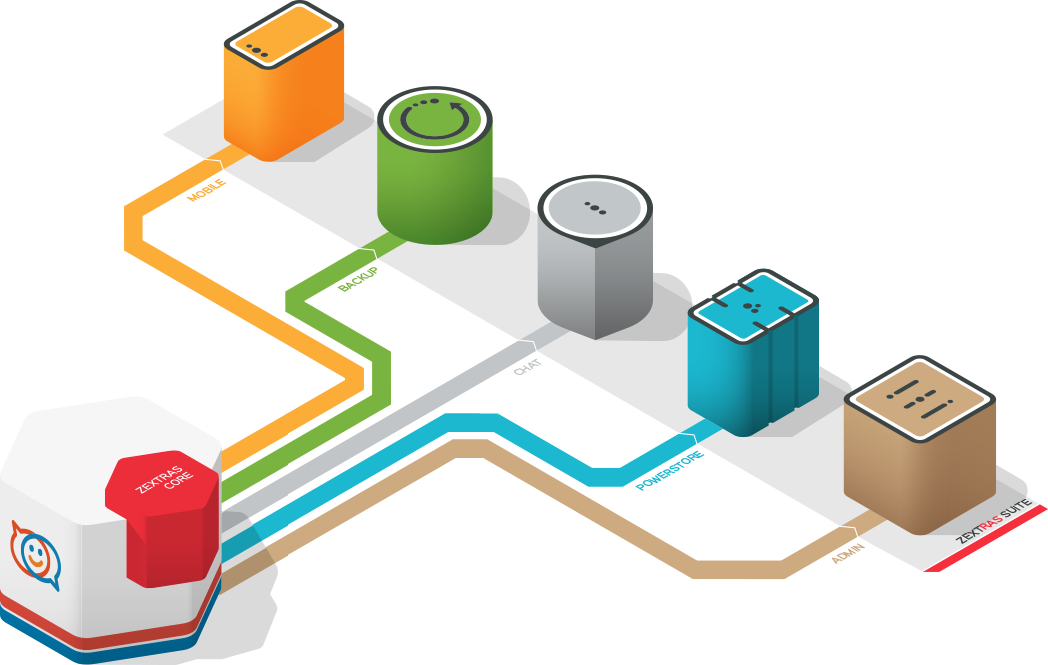
\includegraphics[scale=0.3]{zextras_2018}
	\caption{Rappresentazione Zextras suite}
	\label{fig:modulizextras}
\end{figure}
\postit{Per fare i riferimenti metti una label sulla parte da riferire (dopo la caption) e poi nel resto ref con l'identificativo dato nella label}
Come rappresentato in figura~\ref{fig:modulizextras}, Zextras suite è un'estensione modulare per Zimbra Open Source che può essere applicata secondo le proprie esigenze. Proprio per questo risulta la migliore scelta per un uso professionale di Zimbra.

\section{Metodo di lavoro}
Tecnicamente usano il metodo SCRUM, con la backlog e sprint di due settimane ma forse mi devo informare su come lavorano. \\


\note{Non so se dire e descrivere  la suite Atlassian che viene utilizzata in azienda perchè io non utilizzo solo Jira e BitBucket mentre c'è e utilizzano anche Bamboo e un'altra cosa per i documenti.}
